The simulations were run with porosities of 0\%, 17\%, 33\% and 50\% and cohesive strengths of 1kPa, 10kPa, 100kPa and 1MPa under impact angles of 0 and 45 degrees. This yields 32 simulations in total.

\subsection{Cratering}
- qualitative analysis

- head on
\begin{figure}[H]
   \centering
   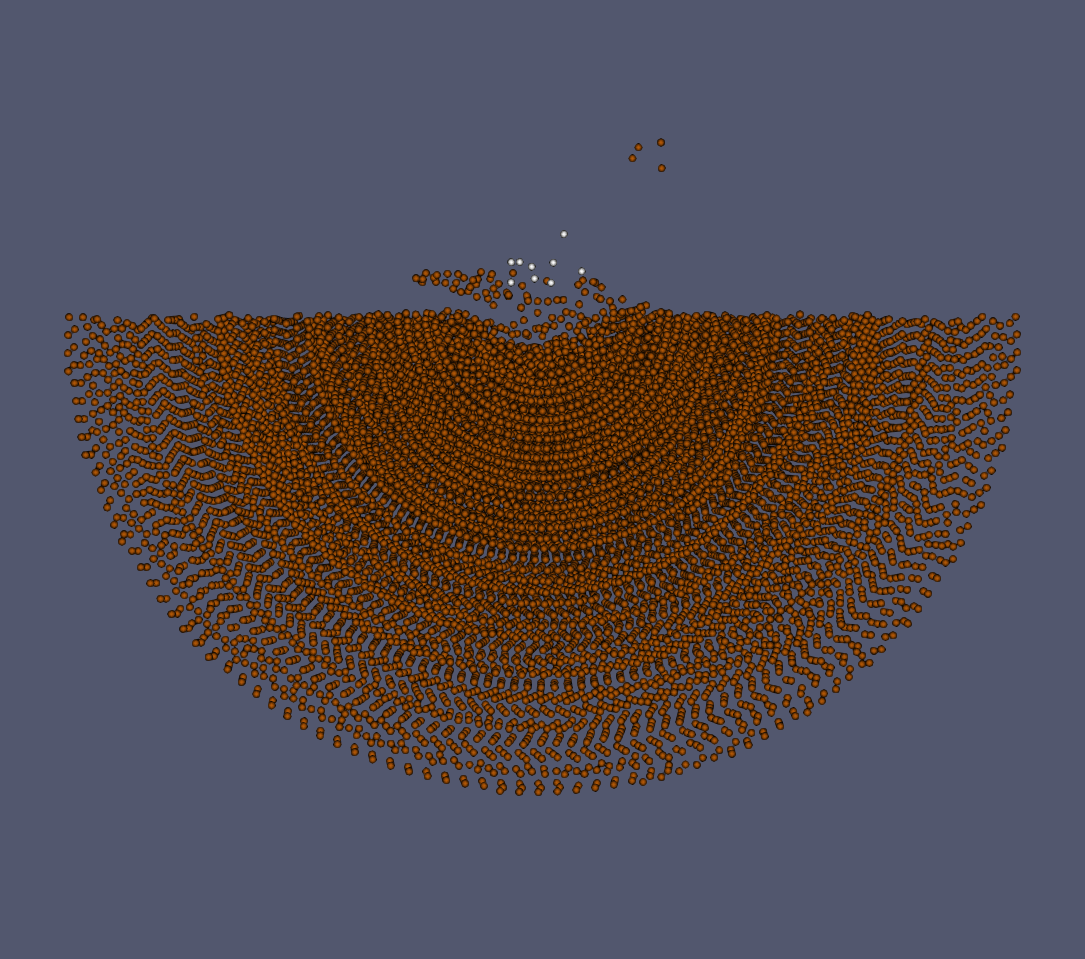
\includegraphics[width=\textwidth]{crater_por0_stre6.png}
   \caption{No porosity (0\%), high strength (Y=1MPa)}
   \label{fig:crater1}
\end{figure}


\begin{figure}[H]
   \centering
   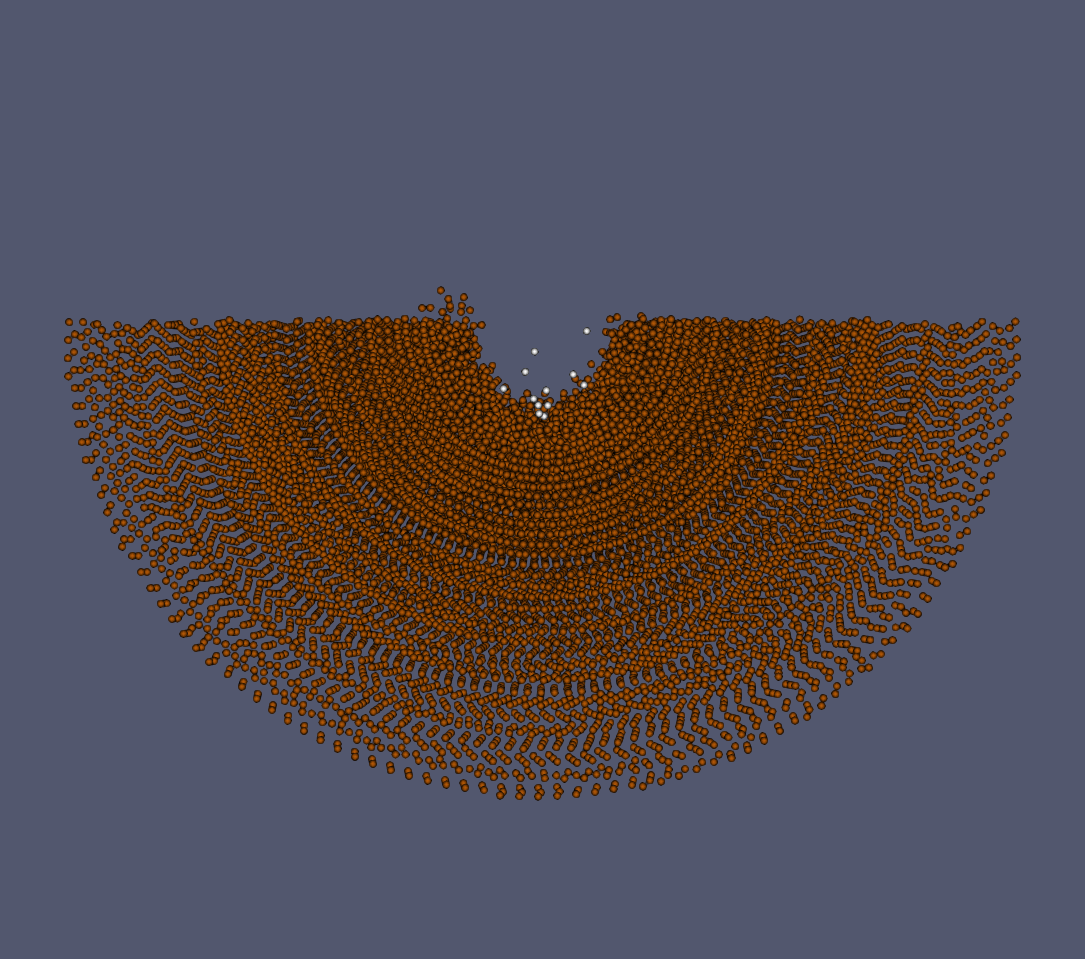
\includegraphics[width=\textwidth]{crater_por50_stre6.png}
   \caption{High porosity (50\%), high strength (Y=1MPa)}
   \label{fig:crater2}
\end{figure}

\begin{figure}[H]
   \centering
   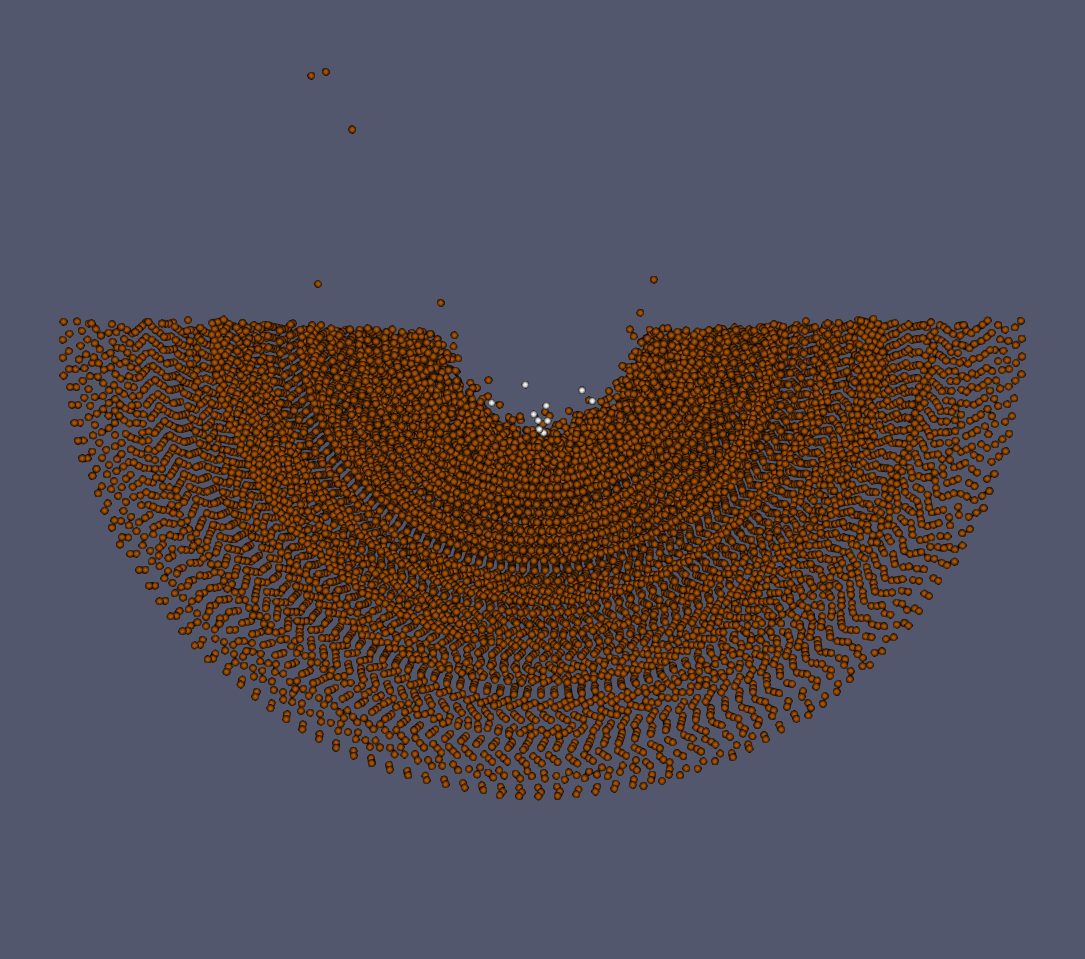
\includegraphics[width=\textwidth]{crater_por50_stre3.png}
   \caption{High porosity (50\%), low strength (Y=1kPa)}
   \label{fig:crater3}
\end{figure}

- 45 degrees
\begin{figure}[H]
   \centering
   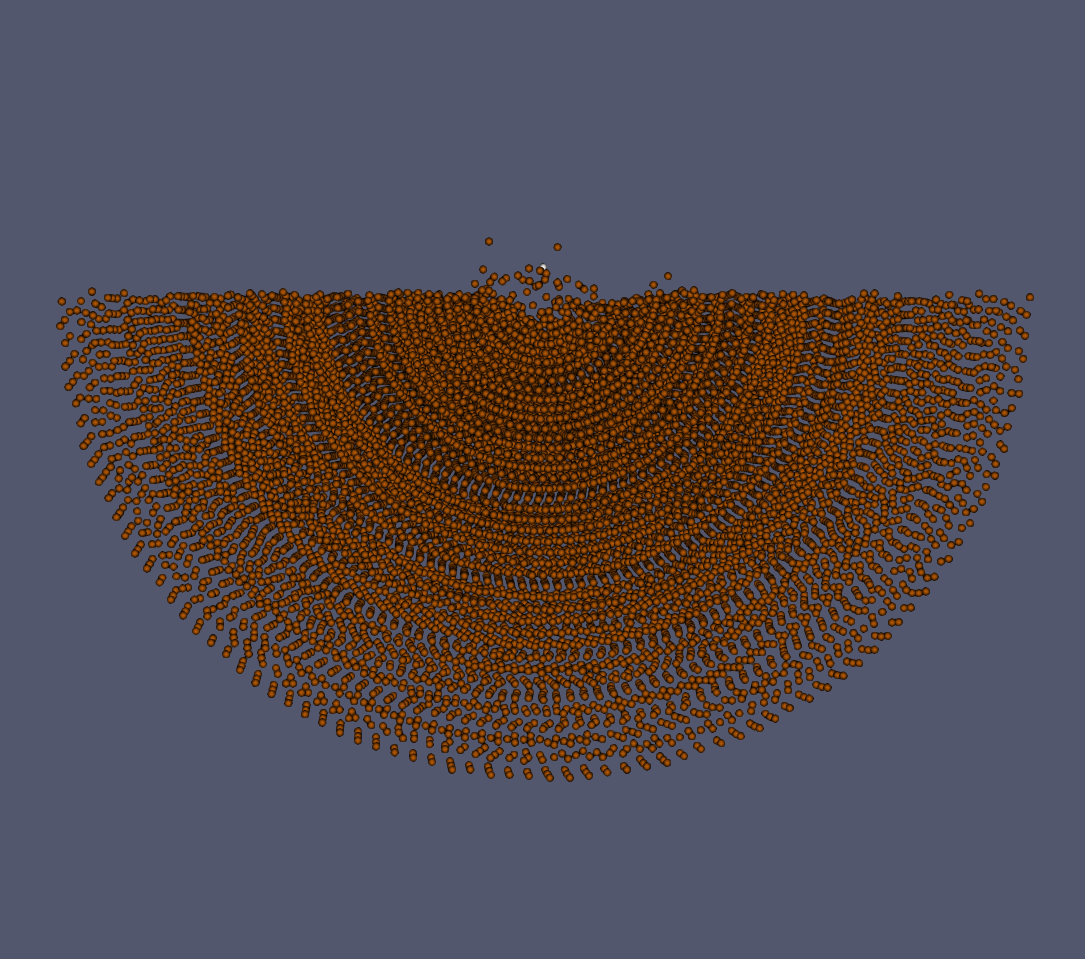
\includegraphics[width=\textwidth]{crater_por0_stre6_ang45.png}
   \caption{No porosity (0\%), high strength (Y=1MPa), 45 degree angle}
   \label{fig:crater4}
\end{figure}


\begin{figure}[H]
   \centering
   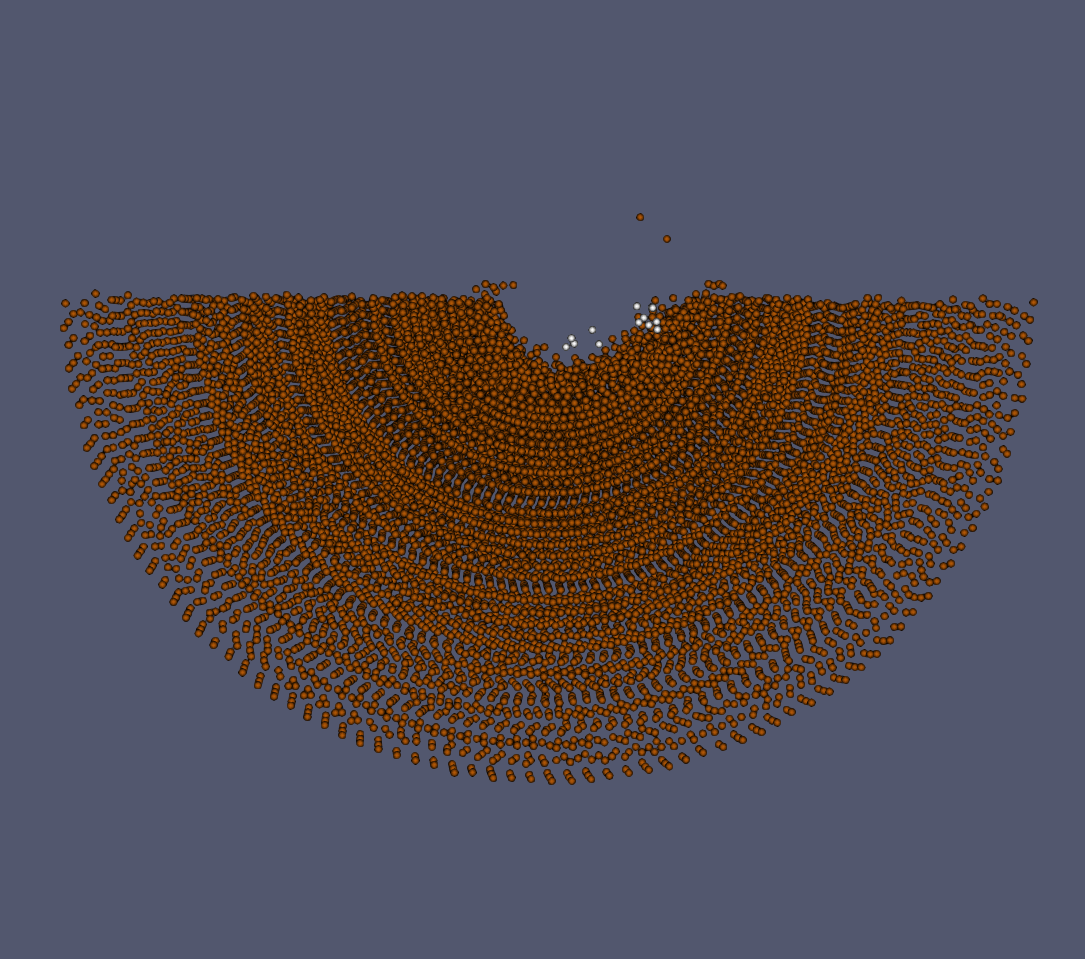
\includegraphics[width=\textwidth]{crater_por50_stre6_ang45.png}
   \caption{High porosity (50\%), high strength (Y=1MPa), 45 degree angle}
   \label{fig:crater5}
\end{figure}

\begin{figure}[H]
   \centering
   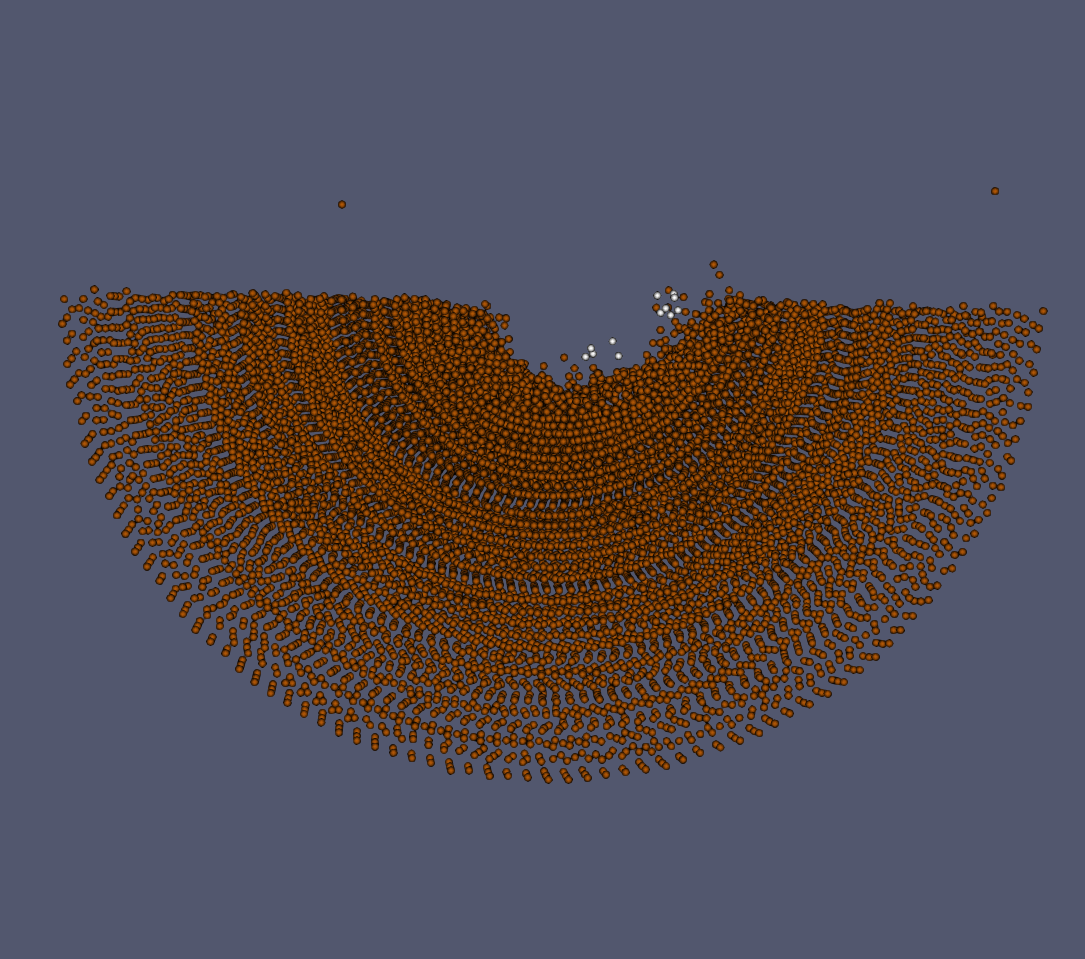
\includegraphics[width=\textwidth]{crater_por50_stre3_ang45.png}
   \caption{High porosity (50\%), low strength (Y=1kPa), 45 degree angle}
   \label{fig:crater6}
\end{figure}

\subsection{Damage}

\subsection{Beta factor}
- explanation of beta factor

\begin{figure}[H]
   \centering
   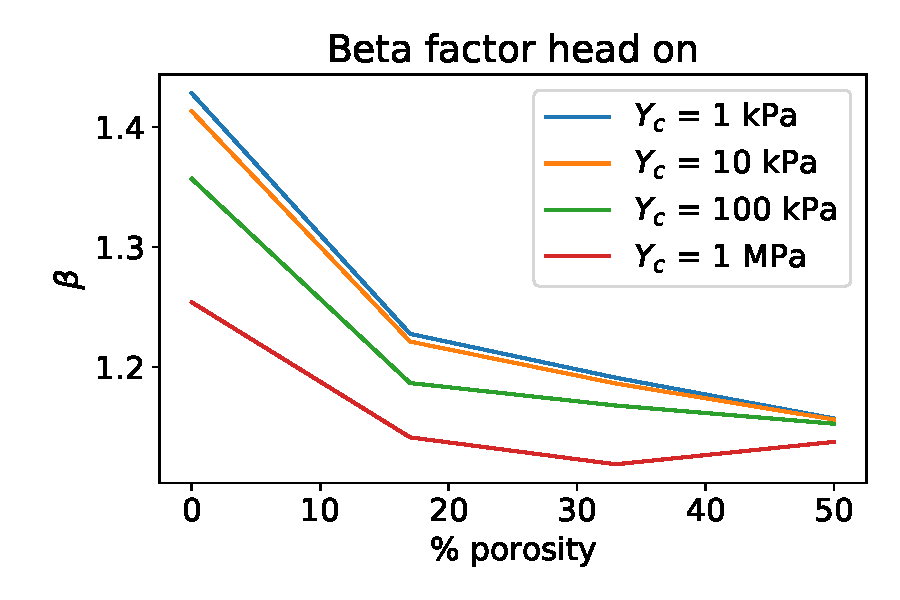
\includegraphics[width=\textwidth]{beta_results_ang0.pdf}
   \caption{beta factor}
   \label{fig:beta_factor_0}
\end{figure}

\begin{figure}[H]
   \centering
   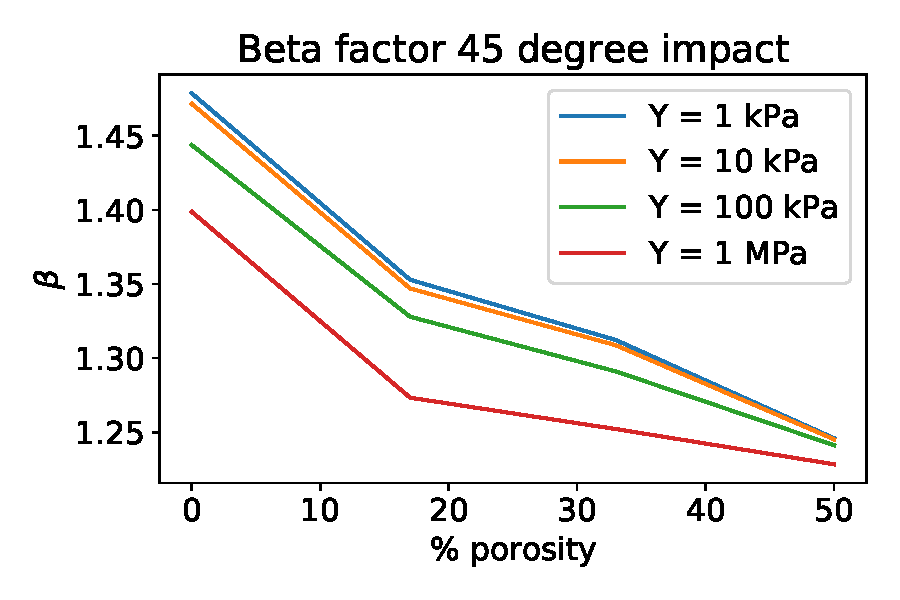
\includegraphics[width=\textwidth]{beta_results_ang45.pdf}
   \caption{beta factor}
   \label{fig:beta_factor_45}
\end{figure}

- only particles with positive velocity along impact direction above escape velocity
\begin{equation}
   v_{esc} = \sqrt{\left(\dfrac{2GM}{r_i}\right)}
\end{equation}
where $M = \frac{4}{3}\pi R^3 \rho_{asteroid}$ is the estimated mass of asteroid with R = 75m and $\rho{asteroid}$ = 2.8$\frac{g}{cm^3}$ and $r_i$ distance of sph particle from center of estimated asteroid sphere
- few particles (with highest velocities so the ones that are far away) account for most of the momentum

\begin{figure}[H]
   \centering
   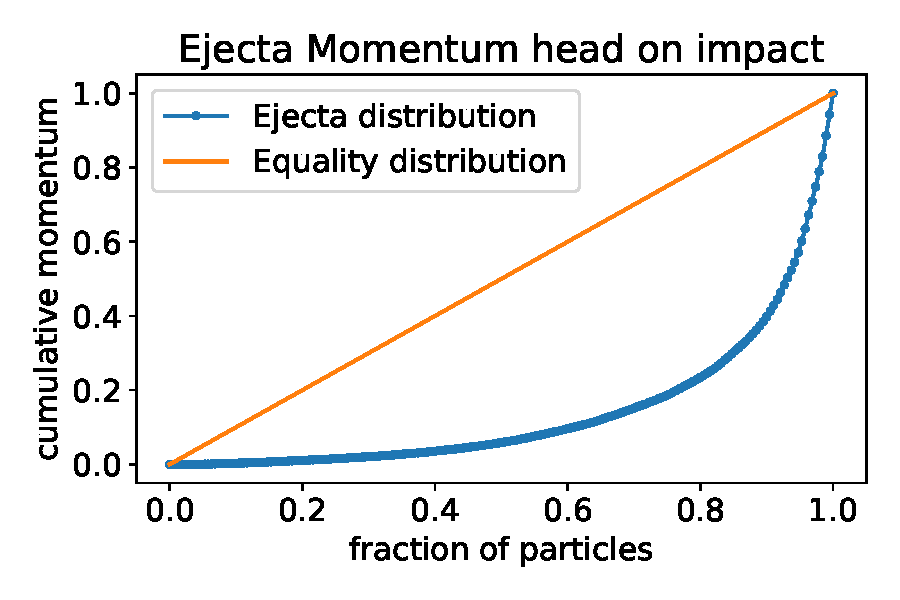
\includegraphics[width=\textwidth]{beta_lorenz_ang0.pdf}
   \caption{Lorenz curve for momentum distribution head on}
   \label{fig:beta_factor_lorenz_0}
\end{figure}

\begin{figure}[H]
   \centering
   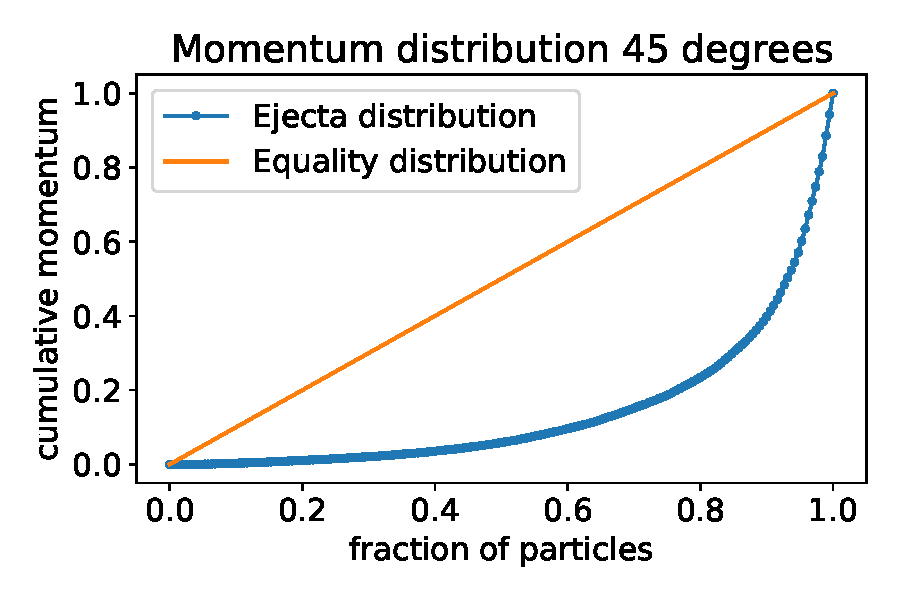
\includegraphics[width=\textwidth]{beta_lorenz_ang45.pdf}
   \caption{Lorenz curve for momentum distribution 45 degree}
   \label{fig:beta_factor_lorenz_45}
\end{figure}